\documentclass{oci}
\usepackage[utf8]{inputenc}
\usepackage{lipsum}
\usepackage{tikz}

\title{Reloj inteligente}

\begin{document}
\begin{problemDescription}
  Nicolás acaba de comprarse un \emph{reloj inteligente}.
  Ahora, cada vez que realiza una actividad deportiva, Nicolás lleva su nuevo
  reloj, pues este le entrega información muy útil como su velocidad o ritmo
  cardíaco.
  Por otro lado, su reloj también se conecta con una aplicación en su celular y
  lleva un registro de todas las actividades que realiza.
  La parte entretenida es que la aplicación propone ciertos desafíos.
  En uno de los desafíos, Nicolás puede escoger un entero $M$ y, entre todas sus
  actividades, la aplicación le dirá el tiempo mínimo en que ha podido recorrer
  $M$ metros.

  Después de un tiempo ocupando la aplicación, Nicolás se ha dado cuenta de que el
  desafío no funciona como él esperaba.
  Cada vez que empieza una actividad, el reloj guarda el tiempo cada $M$
  metros recorridos.
  Por ejemplo, si $M=3$, la aplicación guardará el tiempo que tardó en
  recorrer los primero 3 metros, luego el tiempo entre el metro 3 y
  el 6, entre el 6 y el 9, etc.
  A Nicolás le gustaría que la aplicación considerara todos los intervalos en
  los que recorrió $M$ metros.
  Por ejemplo, para $M=3$, otros intervalos posibles podrían ser entre el
  metro 2 y 5 o entre el 7 y el 10.

  Para suerte de Nicolás, el reloj es realmente inteligente y puede
  programarse para añadir nuevas funcionalidades.
  Lamentablemente, Nicolás es realmente malo programando y necesita de tu ayuda.

  Internamente, el reloj toma una \emph{muestra} cada segundo y registra la
  distancia en metros que fue recorrida durante ese segundo.
  Las muestras son guardadas en un arreglo de enteros de tamaño $N$.
  Un intervalo corresponde a un conjunto consecutivo de muestras y su distancia,
  a la suma total de todas las muestras en él.
  Como es posible que la distancia de los intervalos no sea exactamente $M$,
  a Nicolás le interesan los intervalos que sean lo más cercanos posible a $M$.
  Un \emph{intervalo válido} es uno cuya distancia es mayor o igual que $M$,
  tal que al quitarle la muestra de más a la derecha, la distancia queda menor
  que $M$.
  Dada la descripción de las muestras, tu tarea es determinar el menor tiempo en
  que Nicolás recorrió un intervalo válido.

  La siguiente figura contiene un ejemplo para un arreglo de muestras de tamaño
  $7$.
  Si $M=8$, algunos intervalos válidos son el contenido entre las posiciones 1 y
  4 (distancia $3+2+1+2=8$) y el contenido entre las posiciones 2 y 5 (distancia
  $2+1+2+4=9$).
  Por otro lado, el intervalo contenido entre las posiciones 2 y 6, a pesar de
  tener una distancia mayor que 8, no es válido, pues al sacarle la muestra de más
  a la derecha su distancia todavía es mayor que 8.
  Finalmente, el intervalo válido de menor tiempo es el contenido entre las
  posiciones 4 y 6.

\begin{center}
	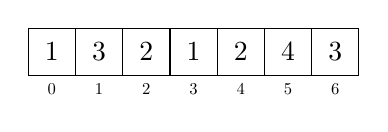
\begin{tikzpicture}[scale = 0.6]
	\foreach \i in {0,...,6}{
		\draw (\i,0) rectangle +(1,1);
		\node at (\i+0.5,-0.3) {\scalebox{0.6}{$\i$}};
	}
	\node at (0+0.5,0.5) {$1$};
	\node at (1+0.5,0.5) {$3$};
	\node at (2+0.5,0.5) {$2$};
	\node at (3+0.5,0.5) {$1$};
	\node at (4+0.5,0.5) {$2$};
	\node at (5+0.5,0.5) {$4$};
	\node at (6+0.5,0.5) {$3$};
	\end{tikzpicture}
\end{center}
\end{problemDescription}

\begin{inputDescription}
  La primera línea de la entrada contiene dos enteros $M$ ($0<M\leq 10^5$) y $N$
  ($N > 0$), correspondientes respectivamente al valor que Nicolás ha escogido
  para el desafío y la cantidad de muestras que registró el reloj.
  La siguiente línea contiene $N$ enteros mayores o iguales que 0 y menores o
  iguales que 100, correspondientes a la cantidad de metros recorridos en cada
  muestra.
\end{inputDescription}

\begin{outputDescription}
  La salida debe contener un único entero correspondiente al tiempo en segundos
  del intervalo válido de menor tiempo.
  Se garantiza que habrá al menos un intervalo válido, es decir, la distancia
  del intervalo formado por todas las muestras será mayor o igual que $M$.
\end{outputDescription}

\begin{scoreDescription}
  \score{20} Se probarán varios casos donde $N\leq 10^2$
  \score{30} Se probarán varios casos donde $N\leq 2\times 10^3$
  \score{50} Se probarán varios casos donde $N\leq 10^6$
\end{scoreDescription}

\begin{sampleDescription}
\sampleIO{sample-1}
\sampleIO{sample-2}
\sampleIO{sample-3}
\end{sampleDescription}

\end{document}
